\newpage
\section{Priors, Regularization, AIC, BIC, LRT}


\subsection{Improper and proper priors}
\no Improper priors are not normalizable, i.e. $\sum_\theta P(\theta) = \infty$
\begin{itemize}
	\item Flat prior: $P(\theta) = \text{const.}$ over any infinite domain.
	\item Uninformative priors (from transformation invariance or max-entropy principles)
	\begin{itemize}
		\item Location parameter: $P(m) = \text{const.}$, on $m \in (-\infty, +\infty)$,
		\item Scale parameter: $P(s) = \frac{\text{const.}}{s}$, on $s\in (0, \infty)$,
		\item Probability parameter: $P(p) = \frac{\text{const.}}{p(1-p)}$, on $p\in(0,1)$.
	\end{itemize}
\end{itemize}
Proper priors are normalized, i.e. $\sum_\theta P(\theta) = 1$.

\subsection{Regularization}
\no Regularized model training
\begin{itemize}
	\item Data: $D$, 
	\item Model: $M$ with parameters $\theta$, likelihood $P(D\;|\;\theta)$
	\item Cost function $= - \log P(D\;|\;\theta) = - L(\theta)$, the log likelihood
	\item Penalty: $\text{penalty}(\theta)$, which is high for implausible $\theta$ values.
	\item Regularized optimum: $\theta_\text{reg.opt.} = \text{arg min}_\theta (-L(\theta) + \text{penalty}(\theta))$
\end{itemize}
Example: Linear regression
\begin{itemize}
	\item Data: $D = \{\;(\{x_{i,k}\}_{k=1}^K, \;y_i)\;\}_{i=1}^N$, where $x_i$ (feature vector) $\in \mathds{R}^K$,  $y_i$ (predicted variable) $\in \mathds{R}$.
	\item Parameters: $\{b_k\}_{k=1}^K$, where $b_k$ (coefficient or weight) $\in \mathds{R}$.
	\item Model:
		\ba
			y_i &=& \sum_{k=1}^K x_{i,k} b_k + \varepsilon_i, \quad \text{with}\quad P(\varepsilon_i) = \text{Normal}(\varepsilon_i\;|\; \mu = 0, \sigma^2 = \sigma^2) \\
			y &=& X b + \varepsilon \\
			&& \text{or equivalently} \\
			P(y\;|\;X, b) &=& \prod_{i=1}^N\text{Normal}\left(y_i\;\big|\;\mu = (X b)_i, \;\sigma^2=\sigma^2\right)
		\ea
	\item Log likelihood: $L(b) = \log P(y\;|\;X, b) = -\frac{N}{2}\log(\sigma^2) - \frac{1}{2\sigma^2} \sum_{i=1}^N \Big[y_i - \sum_{k} x_{i,k} b_k\Big]^2$
	\item Maximum likelihood estimate: $b_\text{MLE} = \text{arg max}_b\; L(b) = (X^\top X)^{-1} X^\top y$, \quad $(\sigma^2)_\text{MLE} = \frac{1}{N}|| y - Xb ||^2$
	\item Regularization:
	\begin{itemize}
		\item ``L1 regularization'': $\text{penalty}(b) = \alpha_1 \sum_k |b_k|$ \\ 
		\quad $\Leftrightarrow$ \quad Laplace prior: $P(b_k) = \text{const.} \times e^{- \alpha_1|b_k|} = \text{Laplace}(b_k\;|\;\text{loc}=0, \text{scale}=1/\alpha_1)$

		\item ``L2 regularization'': $\text{penalty}(b) = \frac{\alpha_2}{2}\sum_k (b_k)^2$ 
		\\ 
		\quad $\Leftrightarrow$ \quad Normal prior: $P(b_k) = \text{const.} \times e^{- \alpha_2(b_k)^2 / 2} = \text{Normal}(b_k\;|\;\mu=0, \sigma^2=1/\alpha_2)$

		\item ``Elastic net regularization'': $\text{penalty}(b) = \alpha_1 \sum_k |b_k| + \frac{\alpha_2}{2}\sum_k (b_k)^2$
	\end{itemize}
	The ``hyperparameters'' $\alpha_1$ and $\alpha_2$ can be optimized using ``Leave-one-out'' or ``M-fold''cross-validation.
\end{itemize}

\subsection{Model comparison with asymptotic metrics}
\no Maximum likelihood results from two models
\begin{itemize}
	\item Data $D = \{x_i\}_{i=1}^N$
	\item Null model: \hspace{6.5mm} $M_0$ with parameters $\theta_0$, and $L_0(\theta_0) = P(D\;|\;\theta_0, M_0)$, \;$\theta_{0, \text{MLE}} = \text{argmax}_{\theta_0} L_0(\theta_0)$
	\item Alternate model: $M_1$ with parameters $\theta_1$, and $L_1(\theta_1) = P(D\;|\;\theta_1, M_1)$, \;$\theta_{1, \text{MLE}} = \text{argmax}_{\theta_1} L_1(\theta_1)$
\end{itemize}
Akaike Information Criterion (AIC)
\begin{itemize}
	\item $\text{AIC}(M_i) = -2\Big[L_i(\theta_{i,\text{MLE}}) - \text{dim}(\theta_i)\Big]$ for both $i=0, 1$ models.
	\item If $\text{AIC}(M_1) < \text{AIC}(M_0)$, then $M_1$  is more plausible.
\end{itemize}
Bayesian Information Criterion (BIC)
\begin{itemize}
	\item $\text{BIC}(M_i) = -2\left[L_i(\theta_{i,\text{MLE}}) - \frac{\ln(N)}{2}\text{dim}(\theta_i)\right]$ for both $i=0, 1$ models.
	\item If $\text{BIC}(M_1) < \text{BIC}(M_0)$, then $M_1$  is more plausible.
\end{itemize}
Likelihood Ratio Test (LRT)
\begin{itemize}
	\item $\text{logLR} = \log\frac{P(D\;|\;M_1, \theta_{1,\text{MLE}})}{P(D\;|\;M_0, \theta_{0,\text{MLE}})} = L_1(\theta_{1,\text{MLE}}) - L_0(\theta_{0,\text{MLE}})$
	\item $\text{LRT pvalue} = 1 - \text{cdf }\chi^2\Big(2\,\text{logRL}\;\Big|\;\text{dof} = \text{dim}(\theta_1) - \text{dim}(\theta_0)\Big)$, where $\text{cdf }\chi^2(\ldots\;|\;\text{dof}=d)$ is the cumulative distribution function of the $\chi^2$ distribution with degrees of freedom $d$.
\end{itemize}
Model evidence
\begin{itemize}
	\item $P(D\;|\;M_i) = \sum_{\theta_i} P(D\;|\;\theta_i, M_i) \approx \exp\left(-\frac{1}{2} \text{ IC}\right)$, 
	\item where IC can be either AIC or BIC (or WAIC, WBIC)
	\item Under uniform prior (i.e. $P(M_0) = P(M_1)$), the posterior probability of the alternate model being correct is
		\be
			 P(M_1\;|\;D) \approx \frac{\exp\left(-\frac{1}{2} \text{ IC}_1\right)}{\exp\left(-\frac{1}{2} \text{ IC}_0\right) + \exp\left(-\frac{1}{2} \text{ IC}_1\right)}
		\ee
\end{itemize}

\newpage
\no Example: Linear regression
\begin{itemize}
	\item Data: $D = \{(x_i, y_i)\}_{i=1}^N$ (generated from $y = 1 - 3x - x^2/2 + x^3 + \varepsilon$ with $\text{std}(\varepsilon) = 2$).
\begin{lstlisting}[language=python]
import numpy as np
from numpy.polynomial.polynomial import polyval
from scipy.stats import norm

c_true = [1, -3, -0.5, 1]
sigma_true = 2
x_data = np.linspace(-3, 3, 20)
y_data = [polyval(x, c_true) + norm.rvs(loc=0, scale=sigma_true) 
          for x in x_data]
\end{lstlisting}
	\begin{figure}[h]
		\centering
		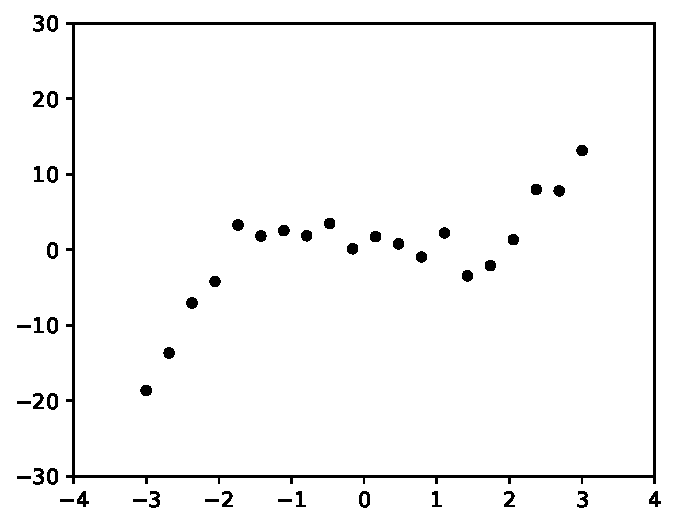
\includegraphics[width=0.4\textwidth]{./figs/03-linear-regression-data.pdf}
	\end{figure}
	\item Models: $M_K:\;K=0,1,2,\ldots$-degree polynomial, parameters: $c = (c_0, c_1, \ldots c_K)$.
	\item ``Linear features'': $X_i := (1, x_i, (x_i)^2, (x_i)^3),\ldots (x_i)^K)$.
\begin{lstlisting}[language=python]
def generate_polynomial_features(x_data, degree):
    K = degree
    N = len(x_data)
    X = np.zeros([N, K+1])
    for i, x in enumerate(x_data):
        for k in range(0, K+1, 1):
            X[i,k] = x**k
    return X
\end{lstlisting}

	\item Likelihood:
	$y = \sum_{k=0}^K X_{i,k} c_k  + \varepsilon$, with $P(\varepsilon) = \text{Normal}(\varepsilon \;|\; 0, \sigma^2)$
\begin{lstlisting}[language=python]
def log_likelihood(X, y, c, sigma2):
    N = len(y_data)
    log_like = 0
    log_like += - N/2.0 * np.log(sigma2)
    log_like += - 1.0/(2 * sigma2) * vector_norm(y - X.dot(c))**2
    return log_like
\end{lstlisting}

\newpage
	\item MLE solution: $c_\text{MLE}= (X^\top X)^{-1} X^\top y$, \quad $(\sigma^2)_\text{MLE} = \frac{1}{N}||y - X c_\text{MLE}||^2$
\begin{lstlisting}[language=python]
def fit_MLE_ploynomial(X, y):
    c_MLE = inv(X.T.dot(X)).dot(X.T).dot(y_data)
    sigma2_MLE = 1.0/len(y) * vector_norm(y - X.dot(c_MLE))**2
    return c_MLE, sigma2_MLE
\end{lstlisting}
	\begin{figure}[h]
		\centering
		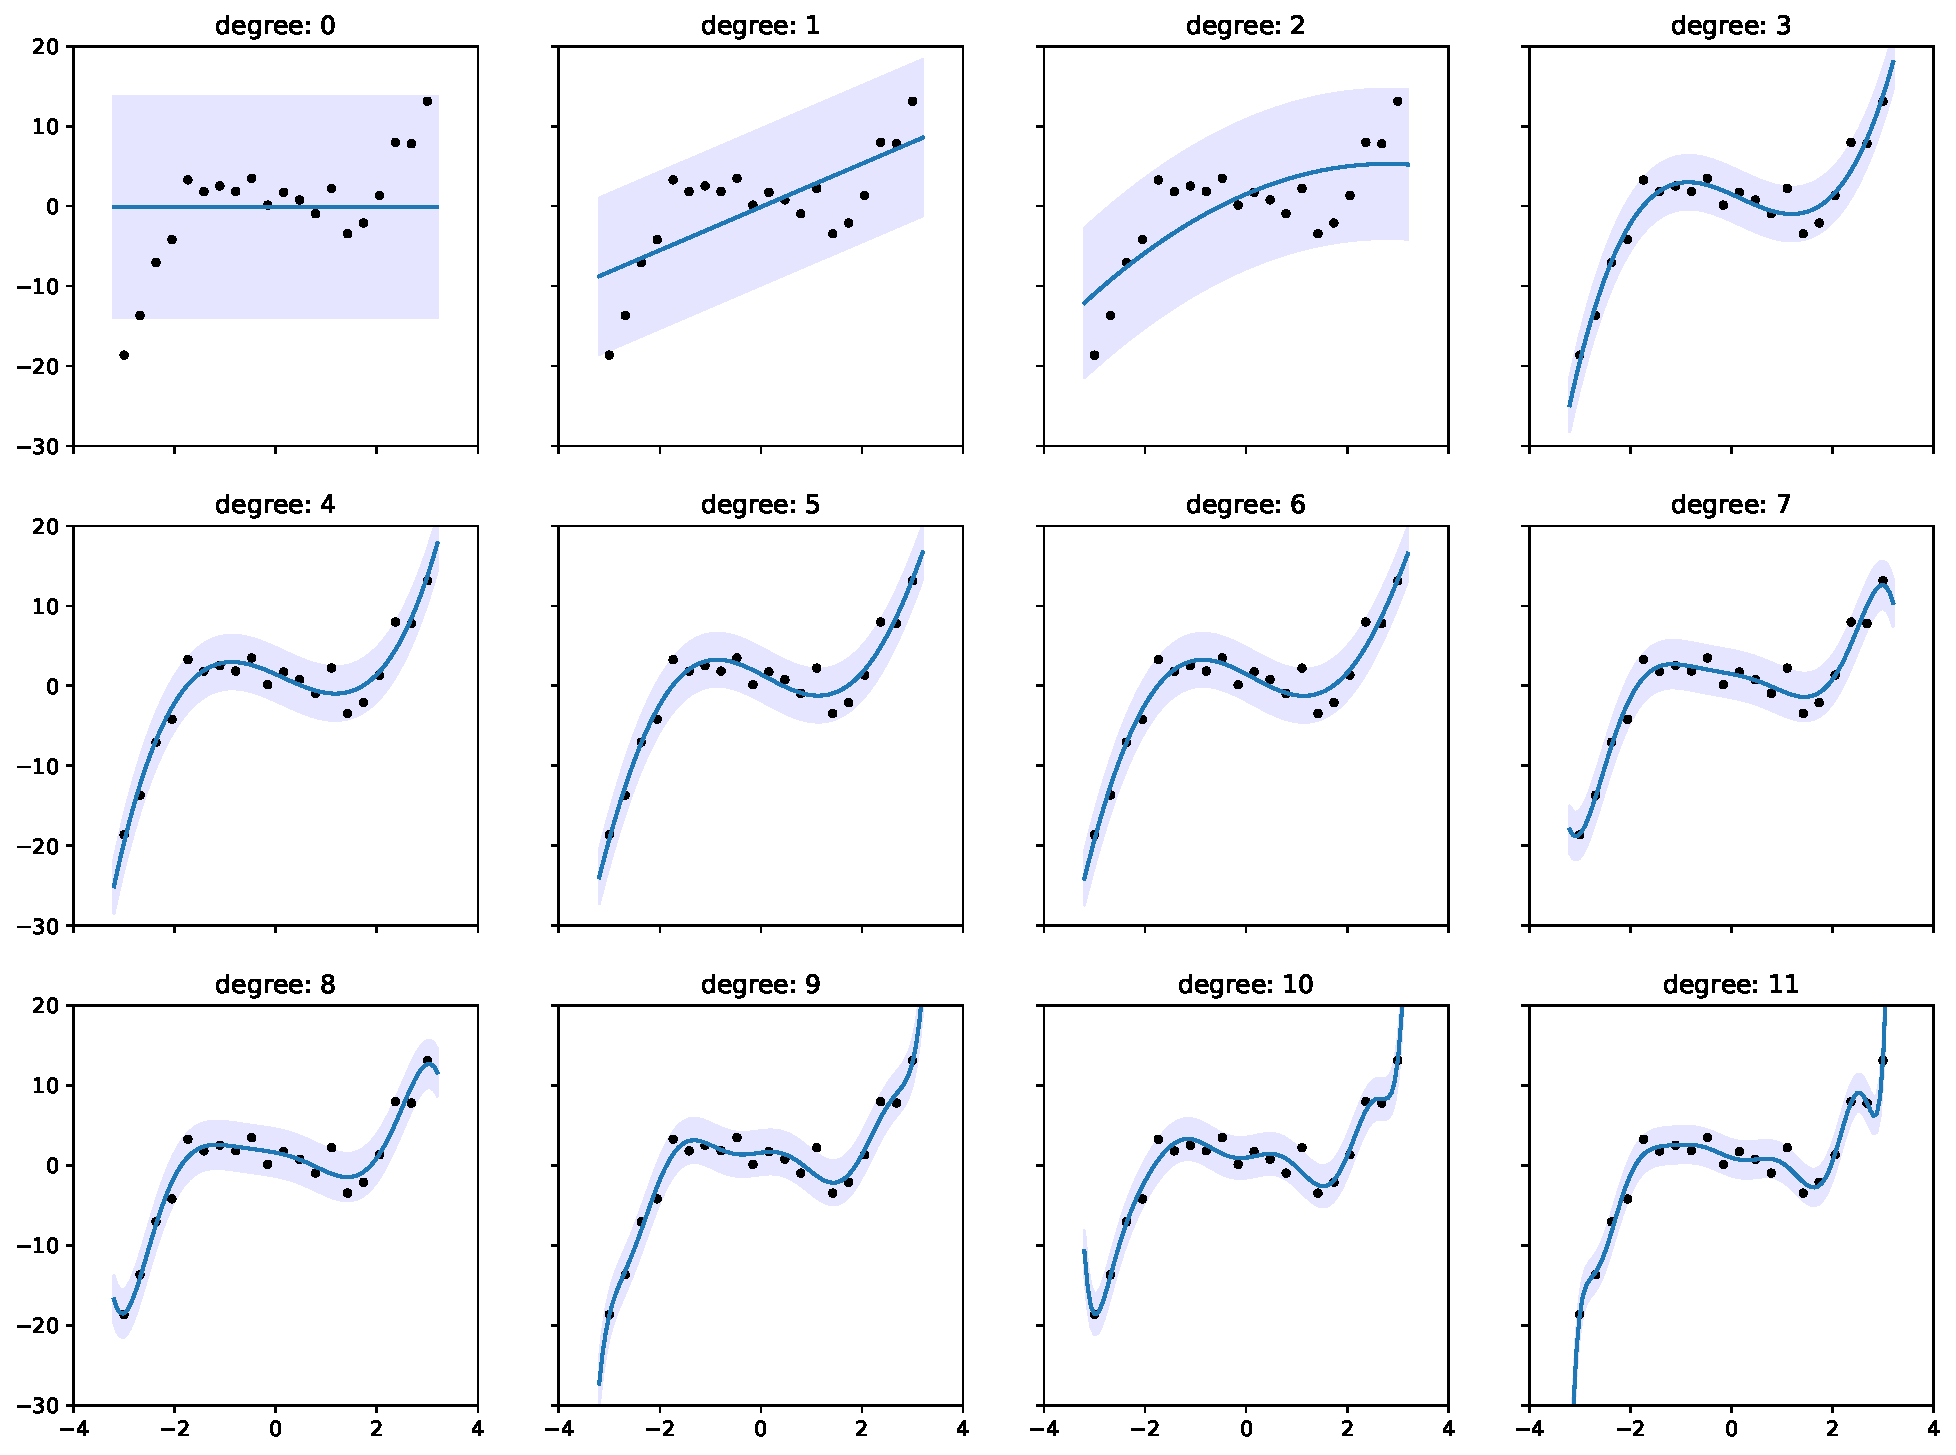
\includegraphics[width=\textwidth]{./figs/03-linear-regression-fits.pdf}
	\end{figure}

\newpage
	\item $\text{AIC}_k = -2 [L_k - (k+2)]$
\begin{lstlisting}[language=python]
def AIC(X, y, c, sigma2):
	dim = len(c) + 1
	loglike = log_likelihood(X, y, c, sigma2)
	return -2 * (loglike - dim)
\end{lstlisting}

	\item $\text{BIC}_k = -2 [L_k - \frac{\log N}{2}(k+2)]$
\begin{lstlisting}[language=python]
def BIC(X, y, c, sigma2):
	N = len(y)
	dim = len(c) + 1
	loglike = log_likelihood(X, y, c, sigma2)
	return -2 * (loglike - np.log(N)/2.0 * dim)
\end{lstlisting}

	\item $\text{LRT pvalue}_{k} = 1 - \text{cdf }\chi^2(2(L_k - L_{k-1})\;|\;\text{dof} = 1)$ \\
	(calculated against the model with one less degree)
\begin{lstlisting}[language=python]
from scipy.stats import chi2

pvalues = [np.nan]
for deg in degrees[1:]:
    L1 = loglikes[deg]
    L0 = loglikes[deg-1]
    logLR = L1 - L0
    dof = 1
    pvalue = chi2.sf(2*logLR, dof)
    pvalues.append(pvalue)
\end{lstlisting}
	\begin{figure}[h]
		\centering
		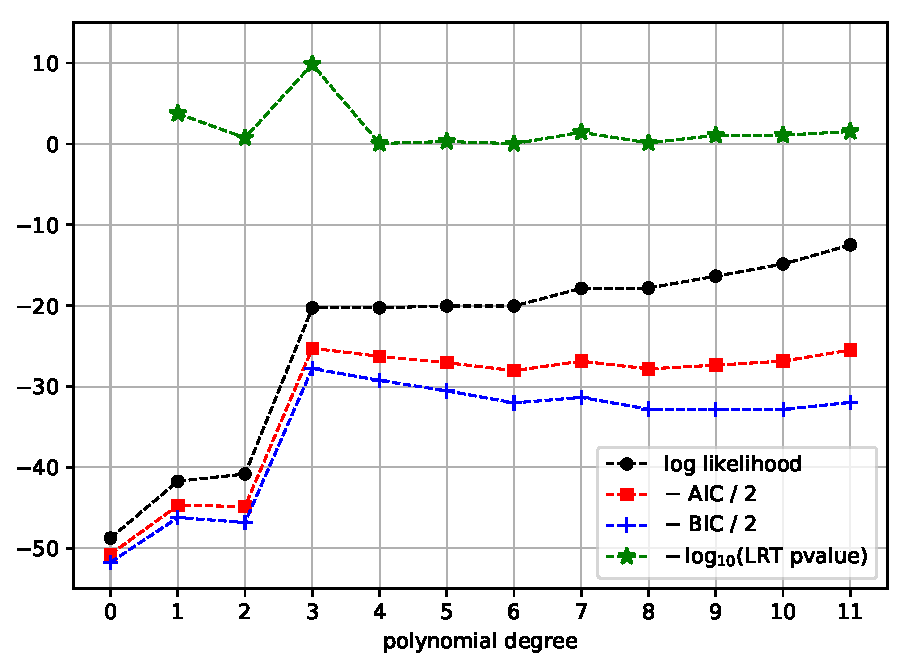
\includegraphics[width=0.75\textwidth]{./figs/03-linear-regression-LL-AIC-BIC-pvalue.pdf}
	\end{figure}

\newpage
\item BIC weights, $P(D\;|\;M_k) \approx e^{-\text{BIC}_k/2} / \sum_{k'=0}^Ke^{-\text{BIC}_{k'}/2}$
\begin{lstlisting}[language=python]
def BIC_weigths(BICs):
	BICs = np.array(BICs)
	w = BICs - np.min(BICs) # for numerical stability
	w = np.exp(-0.5*(w))  
	w /= np.sum(w)
	return w
\end{lstlisting}
	\begin{figure}[h]
		\centering
		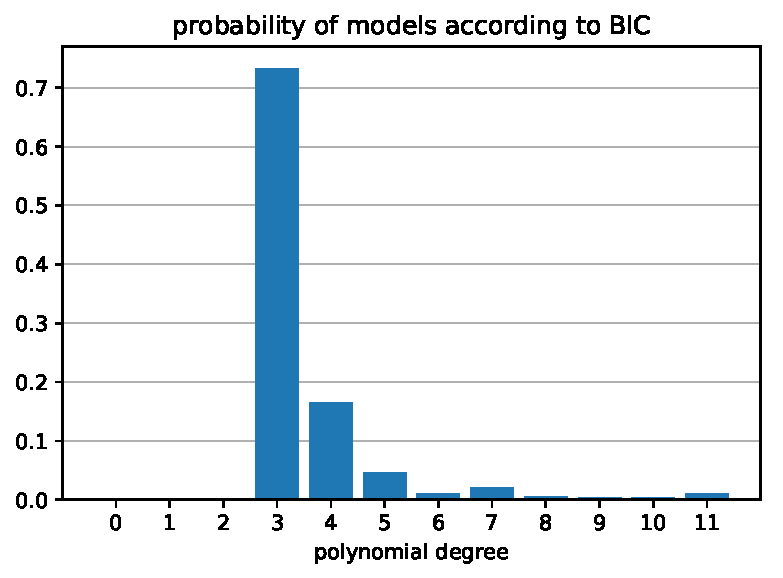
\includegraphics[width=0.7\textwidth]{./figs/03-linear-regression-BIC-weights.pdf}
	\end{figure}
\end{itemize}

